\documentclass[nooutcomes]{ximera}
%\documentclass[space,handout,nooutcomes]{ximera}

% For preamble materials

\usepackage{pgf,tikz}
\usepackage{mathrsfs}
\usetikzlibrary{arrows}
\usepackage{framed}
\usepackage{amsmath}
\pgfplotsset{compat=1.17}

\def\fixnote#1{\begin{framed}{\textcolor{red}{Fix note: #1}}\end{framed}}  % Allows insertion of red notes about needed edits
%\def\fixnote#1{}

\def\detail#1{{\textcolor{blue}{Detail: #1}}}   

\pdfOnly{\renewenvironment{image}[1][]{\begin{center}}{\end{center}}}

\graphicspath{
  {./}
  {chapter1/}
  {chapter2/}
  {chapter4/}
  {proofs/}
  {graphics/}
  {../graphics/}
}

\newenvironment{sectionOutcomes}{}{}


%%% This set of code is all of our user defined commands
\newcommand{\bysame}{\mbox{\rule{3em}{.4pt}}\,}
\newcommand{\N}{\mathbb N}
\newcommand{\C}{\mathbb C}
\newcommand{\W}{\mathbb W}
\newcommand{\Z}{\mathbb Z}
\newcommand{\Q}{\mathbb Q}
\newcommand{\R}{\mathbb R}
\newcommand{\A}{\mathbb A}
\newcommand{\D}{\mathcal D}
\newcommand{\F}{\mathcal F}
\newcommand{\ph}{\varphi}
\newcommand{\ep}{\varepsilon}
\newcommand{\aph}{\alpha}
\newcommand{\QM}{\begin{center}{\huge\textbf{?}}\end{center}}

\renewcommand{\le}{\leqslant}
\renewcommand{\ge}{\geqslant}
\renewcommand{\a}{\wedge}
\renewcommand{\v}{\vee}
\renewcommand{\l}{\ell}
\newcommand{\mat}{\mathsf}
\renewcommand{\vec}{\mathbf}
\renewcommand{\subset}{\subseteq}
\renewcommand{\supset}{\supseteq}
%\renewcommand{\emptyset}{\varnothing}
%\newcommand{\xto}{\xrightarrow}
%\renewcommand{\qedsymbol}{$\blacksquare$}
%\newcommand{\bibname}{References and Further Reading}
%\renewcommand{\bar}{\protect\overline}
%\renewcommand{\hat}{\protect\widehat}
%\renewcommand{\tilde}{\widetilde}
%\newcommand{\tri}{\triangle}
%\newcommand{\minipad}{\vspace{1ex}}
%\newcommand{\leftexp}[2]{{\vphantom{#2}}^{#1}{#2}}

%% More user defined commands
\renewcommand{\epsilon}{\varepsilon}
\renewcommand{\theta}{\vartheta} %% only for kmath
\renewcommand{\l}{\ell}
\renewcommand{\d}{\, d}
\newcommand{\ddx}{\frac{d}{dx}}
\newcommand{\dydx}{\frac{dy}{dx}}


\usepackage{bigstrut}


\title{Constructions}
\author{Bart Snapp and Brad Findell}
\begin{document}
\begin{abstract}
Short-answer questions about how to do constructions. 
\end{abstract}
\maketitle

% What are the rules for compass and straightedge constructions?
% What is a collapsing compass? Why don't we use them or worry about them any more?
% Prove that the collapsing compass is equivalent to the modern compass.
%
%\begin{hint}[Transferring a Segment]\index{compass and straightedge!transferring a segment}
%Given a segment, we wish to move it so that it starts on a given
%point, on a given line.
%\begin{enumerate}        
%\item Draw a line through the point in question.
%\item Open your compass to the length of the line segment and draw a circle with the given point as its center.
%\item The line segment consisting of the given point and the intersection of the circle and the line 
%is the transferred segment.
%\end{enumerate}
%\end{hint}




\begin{problem}
Given a line segment, construct an equilateral triangle whose edge has the length of the given segment. Explain the steps in your construction and how you know it works.

\begin{image}
\definecolor{uuuuuu}{rgb}{0.26666666666666666,0.26666666666666666,0.26666666666666666}
\definecolor{qqqqff}{rgb}{0.,0.,1.}
\begin{tikzpicture}[line cap=round,line join=round,>=triangle 45,x=1.0cm,y=1.0cm]
%\clip(-0.5,3.5) rectangle (4.5,4.5);
\clip(-3,3.5) rectangle (8,4.5);
\draw[color=white] (-3,4) circle (0.2pt);
\draw[color=white] (8,4) circle (0.2pt);
\draw [line width=1.6pt] (0.,4.)-- (2.,4.);
\begin{scriptsize}
\draw [fill=qqqqff] (0.,4.) circle (1.0pt);
\draw[color=qqqqff] (-0.25818181818181923,4.070909090909098) node {$A$};
\draw [fill=qqqqff] (2.,4.) circle (1.0pt);
\draw[color=qqqqff] (2.232727272727274,4.089090909090916) node {$B$};
\end{scriptsize}
\end{tikzpicture}
\end{image}


Which of the following \textbf{best} describes the process: 
\begin{multipleChoice} 
\choice[correct]{Construct two circles, one with each end point as the center and with the other as a point on the circle.}
\choice{Measure a 60 degree angle.}
\choice{Construct a 90 degree angle.}
\choice{Find the midpoint of the segment.}
\end{multipleChoice}
  
\begin{problem}
Correct.  And, as shown below, the two circles intersect at point $C$.  From the construction, $AB = \answer{AC}$ because both are radii of the circle with center $A$.  Similarly, $BA = \answer{BC}$ because radii of the circle with center $\answer{B}$.  Finally, $AC=AB$ because they both equal $\answer{BA}$.  Therefore $\triangle ABC$ is 
$\answer[format=string]{equilateral}$, as desired.  

Notice that we also could have constructed another equilateral triangle, $\triangle \answer{ABD}$, and it is congruent to $\triangle{ABC}$.  

\begin{image}
\definecolor{uuuuuu}{rgb}{0.26666666666666666,0.26666666666666666,0.26666666666666666}
\definecolor{qqqqff}{rgb}{0.,0.,1.}
\begin{tikzpicture}[line cap=round,line join=round,>=triangle 45,x=1.0cm,y=1.0cm]
%\clip(-2.5,1.5) rectangle (4.5,6.5);
\clip(-3,1.5) rectangle (8,6.5);
\draw[color=white] (-3,4) circle (0.2pt);
\draw[color=white] (8,4) circle (0.2pt);
\draw [line width=1.6pt] (0.,4.)-- (2.,4.);
\draw [line width=0.8pt] (0.,4.) circle (2.cm);
\draw [line width=0.8pt] (2.,4.) circle (2.cm);
\draw [line width=1.6pt] (0.,4.)-- (1.,5.732050807568877);
\draw [line width=1.6pt] (1.,5.732050807568877)-- (2.,4.);
%\draw [shift={(2.,4.)},line width=0.8pt]  plot[domain=1.8280586657149969:2.410470502159532,variable=\t]({1.*2.*cos(\t r)+0.*2.*sin(\t r)},{0.*2.*cos(\t r)+1.*2.*sin(\t r)});
%\draw [shift={(0.,4.)},line width=0.8pt]  plot[domain=0.7287273257462467:1.3115827158845068,variable=\t]({1.*2.*cos(\t r)+0.*2.*sin(\t r)},{0.*2.*cos(\t r)+1.*2.*sin(\t r)});
\begin{scriptsize}
\draw [fill=qqqqff] (0.,4.) circle (1.0pt);
\draw[color=qqqqff] (-0.25818181818181923,4.070909090909098) node {$A$};
\draw [fill=qqqqff] (2.,4.) circle (1.0pt);
\draw[color=qqqqff] (2.232727272727274,4.089090909090916) node {$B$};
\draw [fill=uuuuuu] (1.,5.732050807568877) circle (1.0pt);
\draw[color=uuuuuu] (0.9963636363636362,6.089090909090911) node {$C$};
\draw [fill=uuuuuu] (1.,2.267949192431123) circle (1.0pt);
\draw[color=uuuuuu] (0.9963636363636362,2.0345454545454675) node {$D$};
\end{scriptsize}
\end{tikzpicture}
\end{image}

% What to notice:
% Two equilateral triangles are created, but they are congruent, so it doesn't matter which one
% The segment connecting the two vertices is the perpendicular bisector, so it will prove useful for bisecting segments and for creating perpendicular lines.  
% 
\begin{problem}
Which of the following figures illustrates an abbreviated method for constructing an equilateral triangle?
\definecolor{uuuuuu}{rgb}{0.26666666666666666,0.26666666666666666,0.26666666666666666}
\definecolor{qqqqff}{rgb}{0.,0.,1.}
\begin{multipleChoice}
\choice{
%\begin{image}
%\definecolor{uuuuuu}{rgb}{0.26666666666666666,0.26666666666666666,0.26666666666666666}
%\definecolor{qqqqff}{rgb}{0.,0.,1.}
\begin{tikzpicture}[line cap=round,line join=round,>=triangle 45,x=1.0cm,y=1.0cm]
\clip(-0.5,3.9) rectangle (4.6,6.2);
\draw [line width=1.6pt] (0.,4.)-- (2.,4.);
\draw [line width=1.2pt] (0.,4.)-- (1.,5.732050807568877);
\draw [line width=1.2pt] (1.,5.732050807568877)-- (2.,4.);
\draw [line width=0.8pt] (0.5550953933803447,5.475185013173314)-- (1.443720041616383,5.988232693040928);
\draw [line width=0.8pt] (0.5371890492927077,5.999254834543638)-- (1.4473230193813333,5.473788741914348);
%\draw [line width=0.8pt] (0.5418181818181814,5.732050807568877)-- (1.4872727272727275,5.732050807568877);
\begin{scriptsize}
\draw [fill=qqqqff] (0.,4.) circle (1.0pt);
\draw[color=qqqqff] (-0.25818181818181923,4.070909090909098) node {$A$};
\draw [fill=qqqqff] (2.,4.) circle (1.0pt);
\draw[color=qqqqff] (2.232727272727274,4.089090909090916) node {$B$};
\draw [fill=uuuuuu] (1.,5.732050807568877) circle (1.0pt);
\draw[color=uuuuuu] (0.9963636363636362,6.089090909090911) node {$C$};
\end{scriptsize}
\end{tikzpicture}
%\end{image}
}
\choice{
%\begin{image}
%\definecolor{uuuuuu}{rgb}{0.26666666666666666,0.26666666666666666,0.26666666666666666}
%\definecolor{qqqqff}{rgb}{0.,0.,1.}
\begin{tikzpicture}[line cap=round,line join=round,>=triangle 45,x=1.0cm,y=1.0cm]
\clip(-0.5,3.9) rectangle (4.6,6.2);
\draw [line width=1.6pt] (0.,4.)-- (2.,4.);
\draw [line width=1.2pt] (0.,4.)-- (1.,5.732050807568877);
\draw [line width=0.8pt] (1.,4.)-- (1.,5.9);
\draw [line width=1.2pt] (1.,5.732050807568877)-- (2.,4.);
%\draw [line width=0.8pt] (0.5550953933803447,5.475185013173314)-- (1.443720041616383,5.988232693040928);
%\draw [line width=0.8pt] (0.5371890492927077,5.999254834543638)-- (1.4473230193813333,5.473788741914348);
\draw [line width=0.8pt] (0.5418181818181814,5.732050807568877)-- (1.4872727272727275,5.732050807568877);
\begin{scriptsize}
\draw [fill=qqqqff] (0.,4.) circle (1.0pt);
\draw[color=qqqqff] (-0.25818181818181923,4.070909090909098) node {$A$};
\draw [fill=qqqqff] (2.,4.) circle (1.0pt);
\draw[color=qqqqff] (2.232727272727274,4.089090909090916) node {$B$};
\draw [fill=uuuuuu] (1.,5.732050807568877) circle (1.0pt);
\draw[color=uuuuuu] (0.9963636363636362,6.1) node {$C$};
\end{scriptsize}
\end{tikzpicture}
%\end{image}
}
\choice[correct]{
%\begin{image}
\begin{tikzpicture}[line cap=round,line join=round,>=triangle 45,x=1.0cm,y=1.0cm]
\clip(-0.5,3.9) rectangle (4.5,6.2);
\draw [line width=1.6pt] (0.,4.)-- (2.,4.);
%\draw [line width=0.8pt] (0.,4.) circle (2.cm);
%\draw [line width=0.8pt] (2.,4.) circle (2.cm);
\draw [line width=1.2pt] (0.,4.)-- (1.,5.732050807568877);
\draw [line width=1.2pt] (1.,5.732050807568877)-- (2.,4.);
\draw [shift={(2.,4.)},line width=0.8pt]  plot[domain=1.8280586657149969:2.410470502159532,variable=\t]({1.*2.*cos(\t r)+0.*2.*sin(\t r)},{0.*2.*cos(\t r)+1.*2.*sin(\t r)});
\draw [shift={(0.,4.)},line width=0.8pt]  plot[domain=0.7287273257462467:1.3115827158845068,variable=\t]({1.*2.*cos(\t r)+0.*2.*sin(\t r)},{0.*2.*cos(\t r)+1.*2.*sin(\t r)});
\begin{scriptsize}
\draw [fill=qqqqff] (0.,4.) circle (1.0pt);
\draw[color=qqqqff] (-0.25818181818181923,4.070909090909098) node {$A$};
\draw [fill=qqqqff] (2.,4.) circle (1.0pt);
\draw[color=qqqqff] (2.232727272727274,4.089090909090916) node {$B$};
\draw [fill=uuuuuu] (1.,5.732050807568877) circle (1.0pt);
\draw[color=uuuuuu] (0.9963636363636362,6.089090909090911) node {$C$};
%\draw [fill=uuuuuu] (1.,2.267949192431123) circle (1.0pt);
%\draw[color=uuuuuu] (0.9963636363636362,2.0345454545454675) node {$D$};
\end{scriptsize}
\end{tikzpicture}
%\end{image}
}
\choice{
%\begin{image}
\begin{tikzpicture}[line cap=round,line join=round,>=triangle 45,x=1.0cm,y=1.0cm]
\clip(-0.5,3.9) rectangle (4.5,6.2);
\draw [line width=1.6pt] (0.,4.)-- (2.,4.);
%\draw [line width=0.8pt] (0.,4.) circle (2.cm);
%\draw [line width=0.8pt] (2.,4.) circle (2.cm);
\draw [line width=1.2pt] (0.,4.)-- (1.15,5.992);
\draw [line width=1.2pt] (0.85,5.992)-- (2.,4.);
%\draw [shift={(2.,4.)},line width=0.8pt]  plot[domain=1.8280586657149969:2.410470502159532,variable=\t]({1.*2.*cos(\t r)+0.*2.*sin(\t r)},{0.*2.*cos(\t r)+1.*2.*sin(\t r)});
%\draw [shift={(0.,4.)},line width=0.8pt]  plot[domain=0.7287273257462467:1.3115827158845068,variable=\t]({1.*2.*cos(\t r)+0.*2.*sin(\t r)},{0.*2.*cos(\t r)+1.*2.*sin(\t r)});
\begin{scriptsize}
\draw [fill=qqqqff] (0.,4.) circle (1.0pt);
\draw[color=qqqqff] (-0.25818181818181923,4.070909090909098) node {$A$};
\draw [fill=qqqqff] (2.,4.) circle (1.0pt);
\draw[color=qqqqff] (2.232727272727274,4.089090909090916) node {$B$};
\draw [fill=uuuuuu] (1.,5.732050807568877) circle (1.0pt);
\draw[color=uuuuuu] (0.9963636363636362,6.089090909090911) node {$C$};
%\draw [fill=uuuuuu] (1.,2.267949192431123) circle (1.0pt);
%\draw[color=uuuuuu] (0.9963636363636362,2.0345454545454675) node {$D$};
\end{scriptsize}
\end{tikzpicture}
%\end{image}
}
\end{multipleChoice}
\begin{problem}
Correct!  The arcs through $C$ are the important parts of circles with centers at $\answer{A}$ and $\answer{B}$ from the construction above. 
\end{problem}
\end{problem}
\end{problem}
\end{problem}

\begin{problem}
Use a compass and straightedge to bisect a given line segment. % Explain the steps in your construction and how you know it works.

\begin{image}
\definecolor{uuuuuu}{rgb}{0.26666666666666666,0.26666666666666666,0.26666666666666666}
\definecolor{qqqqff}{rgb}{0.,0.,1.}
\begin{tikzpicture}[line cap=round,line join=round,>=triangle 45,x=1.0cm,y=1.0cm]
%\clip(-0.5,3.5) rectangle (4.5,4.5);
\clip(-3,3.5) rectangle (8,4.5);
\draw[color=white] (-3,4) circle (0.2pt);
\draw[color=white] (8,4) circle (0.2pt);
\draw [line width=1.6pt] (0.,4.)-- (2.,4.);
\begin{scriptsize}
\draw [fill=qqqqff] (0.,4.) circle (1.0pt);
\draw[color=qqqqff] (-0.25818181818181923,4.070909090909098) node {$A$};
\draw [fill=qqqqff] (2.,4.) circle (1.0pt);
\draw[color=qqqqff] (2.232727272727274,4.089090909090916) node {$B$};
\end{scriptsize}
\end{tikzpicture}
\end{image}


Which of the following \textbf{best} describes the process: 
\begin{multipleChoice} 
\choice{Measure the segment and divide by two.}
\choice{Construct a 60 degree angle.}
\choice{Construct a 90 degree angle.}
\choice[correct]{Construct two circles, one with each end point as the center and with the other as a point on the circle.}
\choice{Construct an isosceles triangle.}
\end{multipleChoice}

\begin{problem}
Correct!  This problem takes advantage of the symmetry in the equilateral triangle construction.  But this time, draw segment $\answer{CD}$ connecting the two intersections of the circles.  That segment intersects $\overline{AB}$ at its midpoint $\answer{M}$.  In fact, that segment is the $\answer[format=string]{perpendicular bisector}$ (two words) of $\overline{AB}$!  You will find that this construction serves many purposes!  

\begin{image}
\definecolor{uuuuuu}{rgb}{0.26666666666666666,0.26666666666666666,0.26666666666666666}
\definecolor{qqqqff}{rgb}{0.,0.,1.}
\begin{tikzpicture}[line cap=round,line join=round,>=triangle 45,x=1.0cm,y=1.0cm]
%\clip(-2.5,1.5) rectangle (4.5,6.5);
\clip(-3,1.5) rectangle (8,6.5);
\draw[color=white] (-3,4) circle (0.2pt);
\draw[color=white] (8,4) circle (0.2pt);
\draw [line width=1.6pt] (0.,4.)-- (2.,4.);
\draw [line width=0.8pt] (0.,4.) circle (2.cm);
\draw [line width=0.8pt] (2.,4.) circle (2.cm);
\draw [line width=0.8pt] (1.,2.267949192431123) -- (1.,5.732050807568877);
%\draw [line width=1.6pt] (0.,4.)-- (1.,5.732050807568877);
%\draw [line width=1.6pt] (1.,5.732050807568877)-- (2.,4.);
%\draw [shift={(2.,4.)},line width=0.8pt]  plot[domain=1.8280586657149969:2.410470502159532,variable=\t]({1.*2.*cos(\t r)+0.*2.*sin(\t r)},{0.*2.*cos(\t r)+1.*2.*sin(\t r)});
%\draw [shift={(0.,4.)},line width=0.8pt]  plot[domain=0.7287273257462467:1.3115827158845068,variable=\t]({1.*2.*cos(\t r)+0.*2.*sin(\t r)},{0.*2.*cos(\t r)+1.*2.*sin(\t r)});
\begin{scriptsize}
\draw [fill=qqqqff] (0.,4.) circle (1.0pt);
\draw[color=qqqqff] (-0.25818181818181923,4.070909090909098) node {$A$};
\draw [fill=qqqqff] (2.,4.) circle (1.0pt);
\draw[color=qqqqff] (2.232727272727274,4.089090909090916) node {$B$};
\draw [fill=uuuuuu] (1.,5.732050807568877) circle (1.0pt);
\draw[color=uuuuuu] (0.9963636363636362,6.089090909090911) node {$C$};
\draw [fill=uuuuuu] (1.,2.267949192431123) circle (1.0pt);
\draw[color=uuuuuu] (0.9963636363636362,2.0345454545454675) node {$D$};
\draw [fill=uuuuuu] (1.,4) circle (1.4pt);
\draw[color=uuuuuu] (1.2,3.85) node {$M$};
\end{scriptsize}
\end{tikzpicture}
\end{image}


%\begin{freeResponse}
%\begin{hint}
%%Given a segment, we wish to cut it in half.
%\begin{enumerate}
%%\item Open your compass to the width of the segment.
%\item Draw two circles, one with each end point as the center and with the other as a point on the circle. 
%\item The circles intersect at two points.  Draw a line through these two points.
%\item The new line bisects the original line segment.
%\end{enumerate}
%\begin{image}
%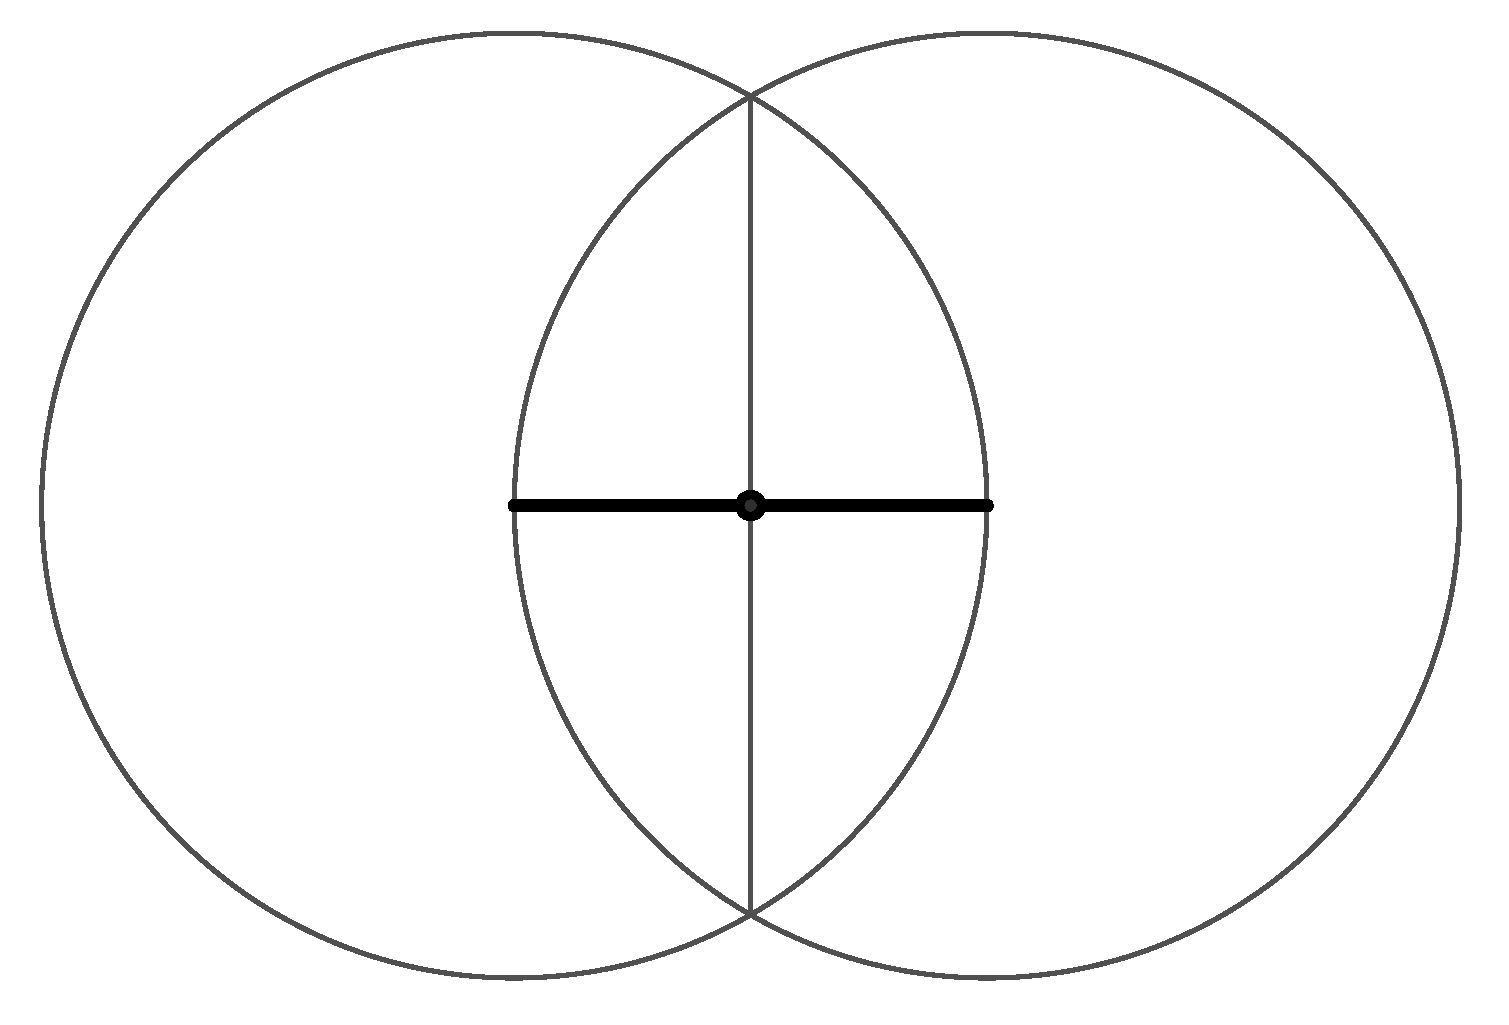
\includegraphics{bisectseg.png}
%\end{image}
%\end{hint}
%\end{freeResponse}
\end{problem}
\end{problem}


%\begin{problem}
%Given a line segment with a point on it, construct a line perpendicular to the segment that passes through the given point. Explain the steps in your construction and how you know it works.
%\begin{freeResponse}
%\begin{hint}
%\begin{enumerate}
%\item With an arbitrary radius, draw a circle to identify two points on the given line equidistant from the given point. 
%\item Now (as above) bisect the segment defined by those two new points. 
%\end{enumerate}
%\begin{image}
%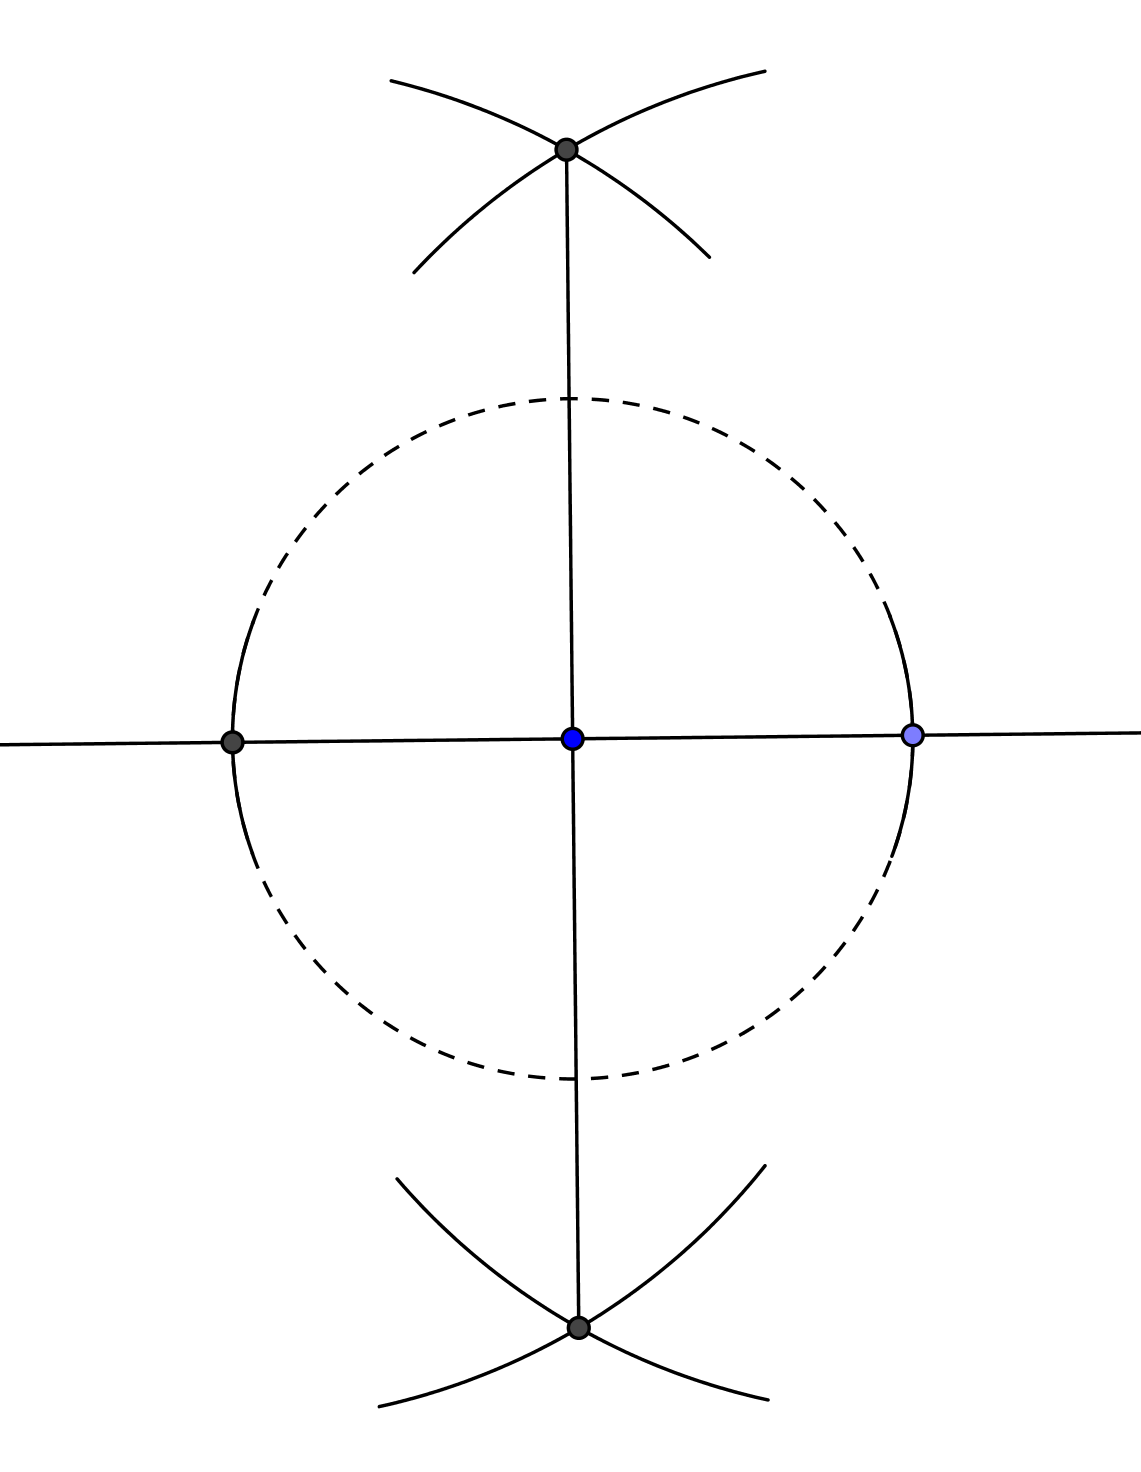
\includegraphics{perpOnLine.png}
%\end{image}
%\end{hint}
%\end{freeResponse}
%\end{problem}


\begin{problem}
Consider the construction below.  
\begin{image}
\definecolor{uuuuuu}{rgb}{0.26666666666666666,0.26666666666666666,0.26666666666666666}
\definecolor{qqqqff}{rgb}{0.,0.,1.}
\begin{tikzpicture}[line cap=round,line join=round,>=triangle 45,x=1.0cm,y=1.0cm]
\clip(-2.58,-1.42) rectangle (8.66,5.84);
\draw[color=white] (-3,4) circle (0.2pt);
\draw[color=white] (8,4) circle (0.2pt);
\draw [line width=0.8pt,domain=1.0:8.660000000000005] plot(\x,{(--4.--2.*\x)/3.});
\draw [line width=0.8pt,domain=1.0:8.660000000000005] plot(\x,{(--5.86-0.3*\x)/2.78});
\draw [line width=0.8pt] (1.,2.) circle (2.796140196771256cm);
\draw [line width=0.8pt] (3.78,1.7) circle (1.905756791286773cm);
\draw [line width=0.8pt] (3.3265292737334002,3.551019515822267) circle (1.905756791286773cm);
\draw [line width=0.8pt,dash pattern=on 2pt off 2pt,domain=1.0:8.660000000000005] plot(\x,{(--7.294362194208519--1.0182269267305872*\x)/4.156294560469553});
\begin{scriptsize}
\draw [fill=qqqqff] (1.,2.) circle (1.5pt);
\draw[color=qqqqff] (0.7,2.29) node {$A$};
\draw [fill=qqqqff] (3.78,1.7) circle (1.5pt);
\draw[color=qqqqff] (3.92,1.51) node {$C$};
\draw [fill=uuuuuu] (3.3265292737334002,3.551019515822267) circle (1.5pt);
\draw[color=uuuuuu] (3.42,4.05) node {$D$};
\draw [fill=uuuuuu] (5.156294560469553,3.0182269267305872) circle (1.5pt);
\draw[color=uuuuuu] (5.36,3.27) node {$E$};
\end{scriptsize}
\end{tikzpicture}
\end{image}
This construction $\answer[format=string]{bisects} \angle A$.  
\begin{problem}
Correct!  The construction works because $AD=\answer{AC}$, 
$DE=\answer{CE}$, and $AE=\answer{AE}$ so that $\triangle ADE \cong \triangle \answer[format=string]{ACE}$ 
by $\answer[format=string]{SSS}$.   Then $\angle DAE\cong \angle \answer[format=string]{CAE}$ from the congruent triangles.  

Note also that quadrilateral $ACED$ is a $\answer[format=string]{kite}$.  Furthermore, if we were to draw $\overline{DC}$, then $\overrightarrow{AE}$ would be its
$\answer[format=string]{perpendicular bisector}$.

\end{problem}
\end{problem}

%
%\begin{problem}
%Use a compass and straightedge to bisect a given angle. Explain the steps in your construction and how you know it works.
%\begin{freeResponse}
%\begin{hint} 
%%We wish to divide an angle in half.
%\begin{enumerate}
%\item Draw a circle with its center being the vertex of the 
%angle.
%%\item Draw a line segment where the circle intersects the lines.
%%\item Bisect the new line segment.  The bisector will bisect the angle.
%\item At each of the points where that circle intersects the sides of the angle, draw a circle with the same radius.
%\item The two circles intersect in two points.  Draw a ray from the vertex of the angle through one of those points.  
%\item The line bisects the angle.  
%\end{enumerate}
%\begin{image}
%
\includegraphics{bisectangle2.png}
%\end{image}
%\end{hint}
%\end{freeResponse}
%\end{problem}
%




\begin{problem}
Given a point and line, construct a line perpendicular to the given line that passes through the given point. Explain the steps in your construction and how you know it works.
\begin{freeResponse}
\begin{hint} 
%Given a point and a line, we wish to construct a line perpendicular to
the original line that passes through the given point.
\begin{enumerate}
\item Draw a circle centered at the point large enough  
       to intersect the line in two distinct points.
\item Bisect the line segment. The line used to do this 
       will be the desired line.
\end{enumerate}
\begin{image}
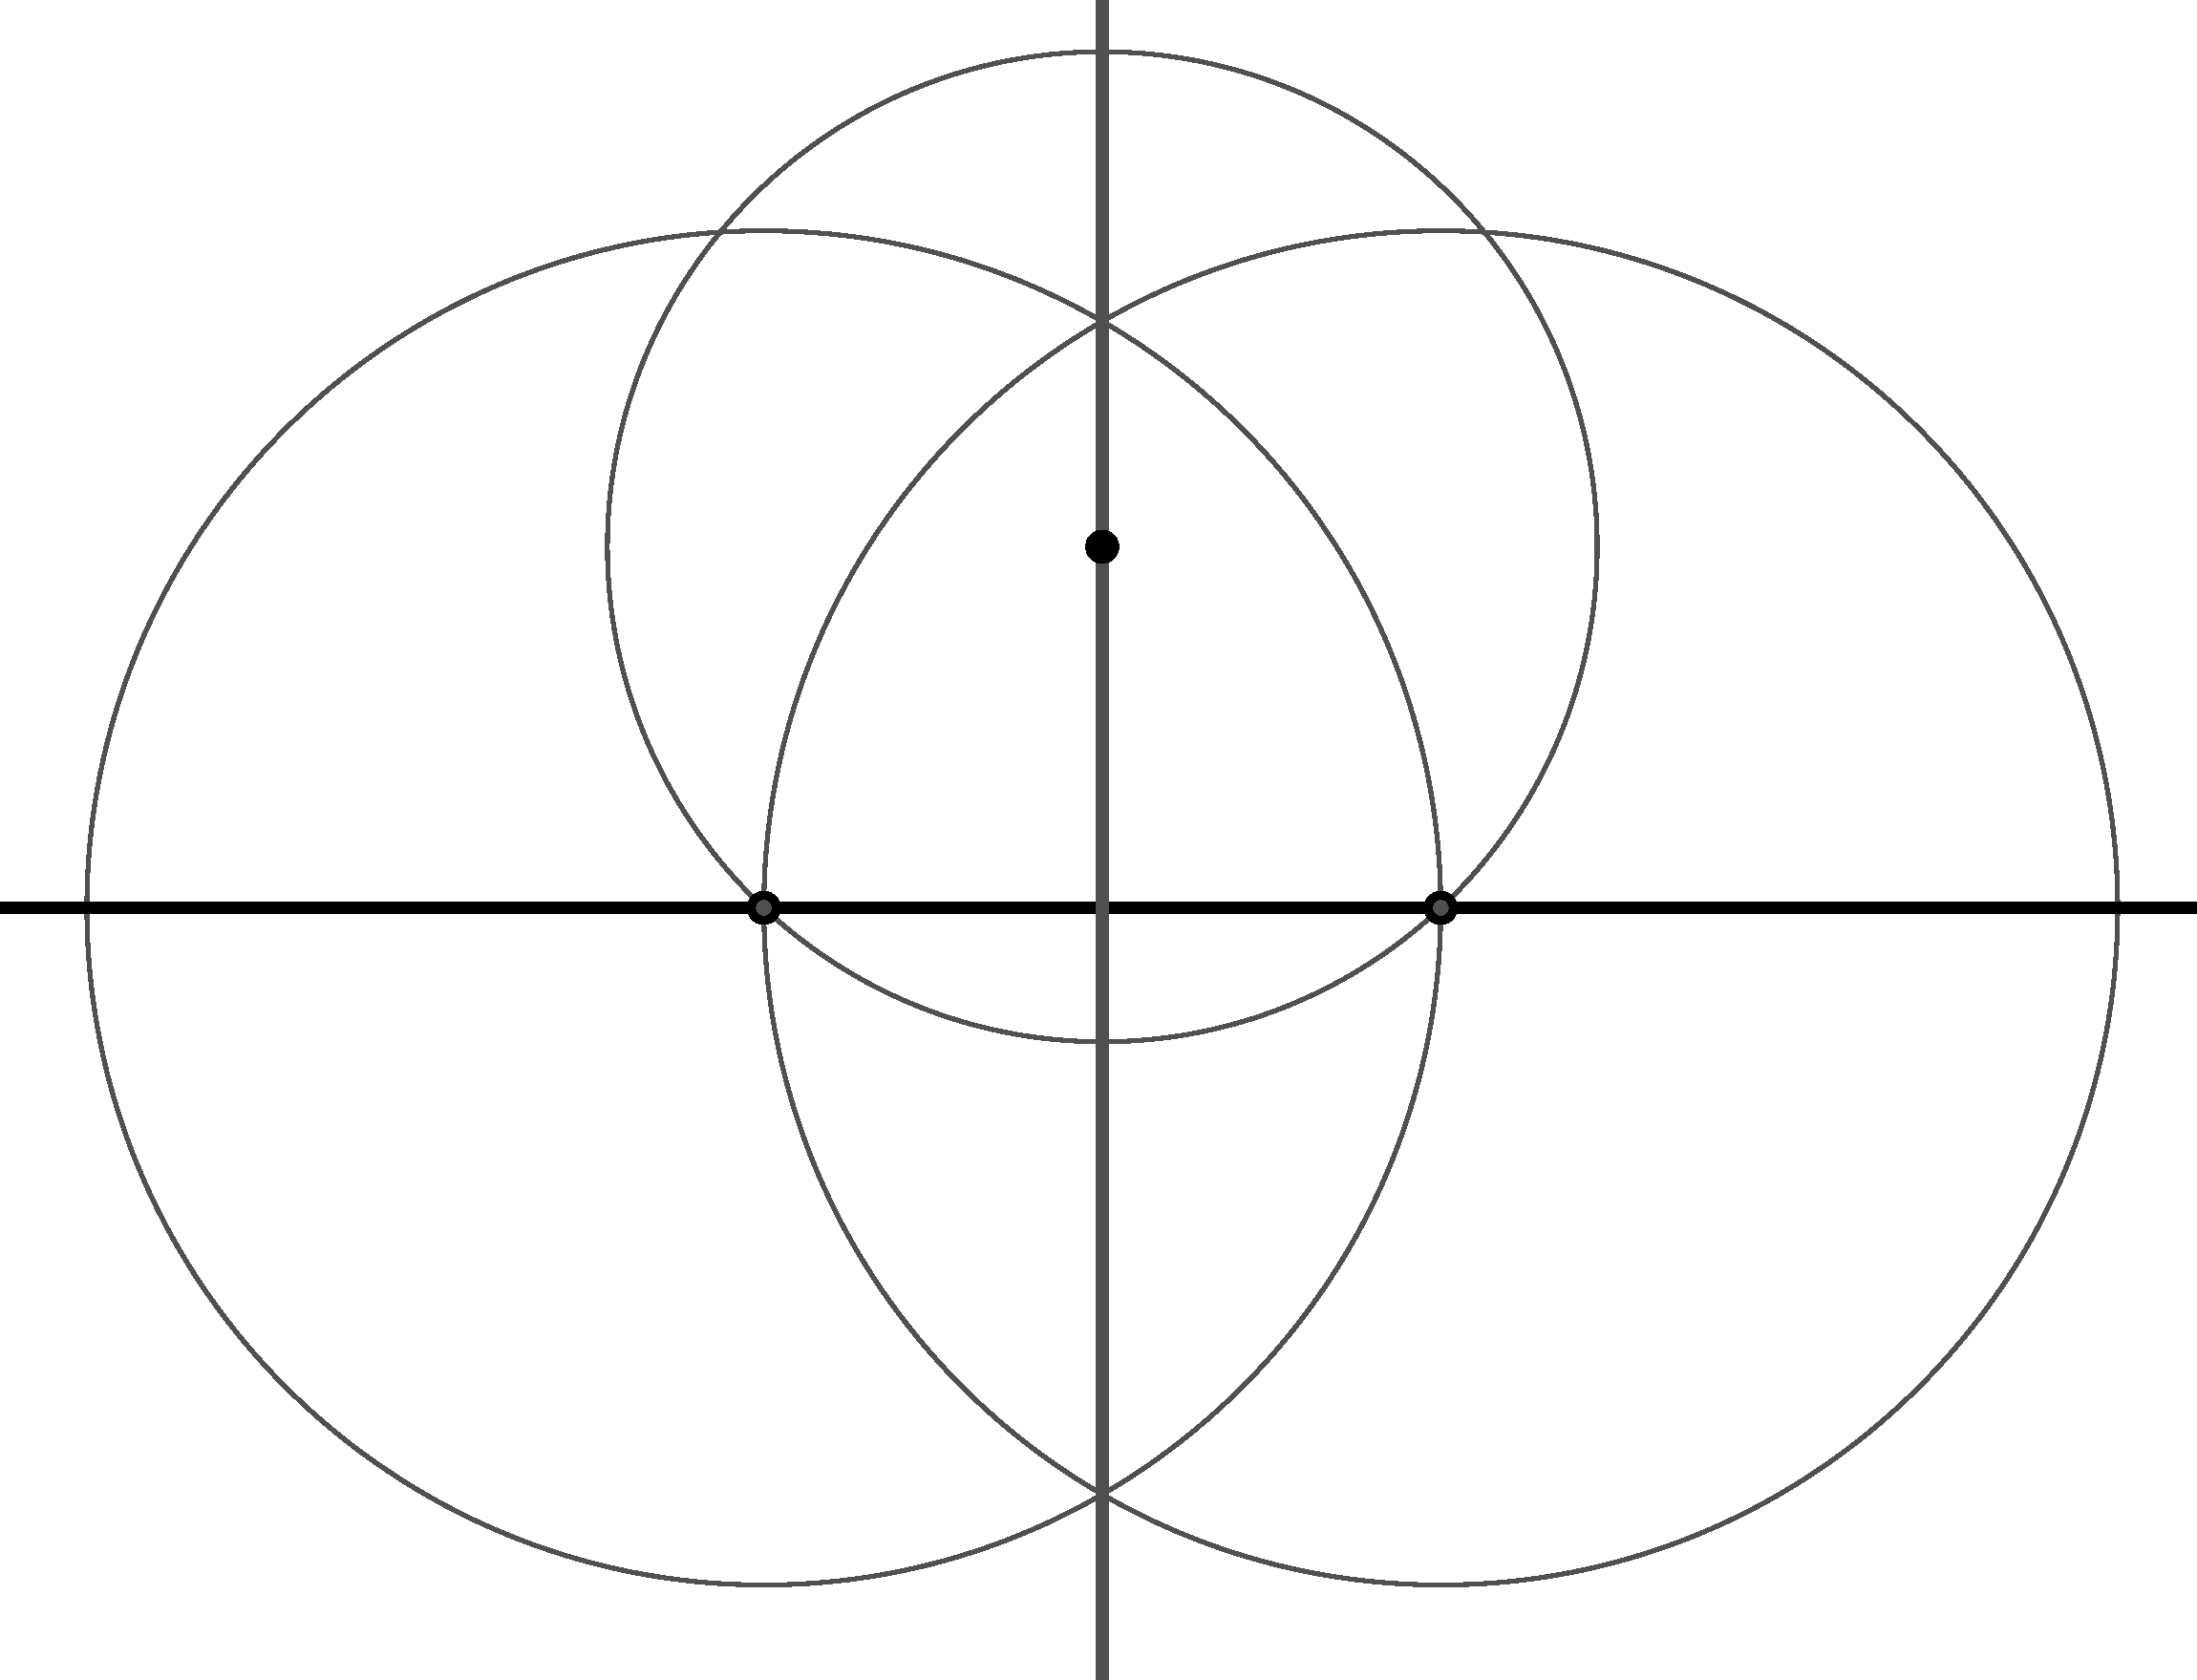
\includegraphics{perpfrompoint.png}
\end{image}
\end{hint}
\end{freeResponse}
\end{problem}

\begin{problem}
Given a point and line, construct a line parallel to the given line that passes through the given point. Explain the steps in your construction and how you know it works.
\begin{freeResponse}
\begin{hint}
Through the given point, construct a perpendicular to the given line.  Then through the same point, construct a perpendicular to the new line. 
\end{hint}
\end{freeResponse}
\end{problem}

%\begin{hint}%[Parallel to a Line through a Point]\index{compass and straightedge!parallel to a line through a point} 
% Given a line and a point, we wish to construct another line parallel
% to the first that passes through the given point.
%\begin{enumerate}
%\item Draw a circle centered at the given point and passing through the given line at two points.
%\item We now have an isosceles triangle, duplicate this triangle.
%\item Connect the top vertexes of the triangles and we get a parallel line.
%\end{enumerate}
%\begin{image}
%\includegraphics{parallel.pdf}
%\end{image}
%\end{hint}

\begin{problem}
Given an angle and a ray, use a compass and straightedge to copy the angle so that the new angle has the a ray as one side. Explain the steps in your construction and how you know it works.
\begin{freeResponse}
\begin{hint}
On the angle, create a triangle.  Then copy the triangle by copying its three sides.  
%Given a point on a line and some angle, we wish to copy the 
%given angle so that the new angle has the point as its 
%vertex and the line as one of its edges.
%\begin{enumerate}
%\item Open the compass to a fixed width and make a circle 
%centered at the vertex of the angle.
%\item Make a circle of the same radius on the line with the point [or on the ray].
%\item Open the compass so that one end touches the first circle 
%where it hits one side of the original angle, with the other end of the compass extended to where the first circle hits the other side of the original angle.
%\item Draw a circle with the radius found above with its center 
%where the second circle hits the line.
%\item Connect the point to where the circles meet. This is the other side of the angle we are constructing.
%\end{enumerate}
%\begin{image}
%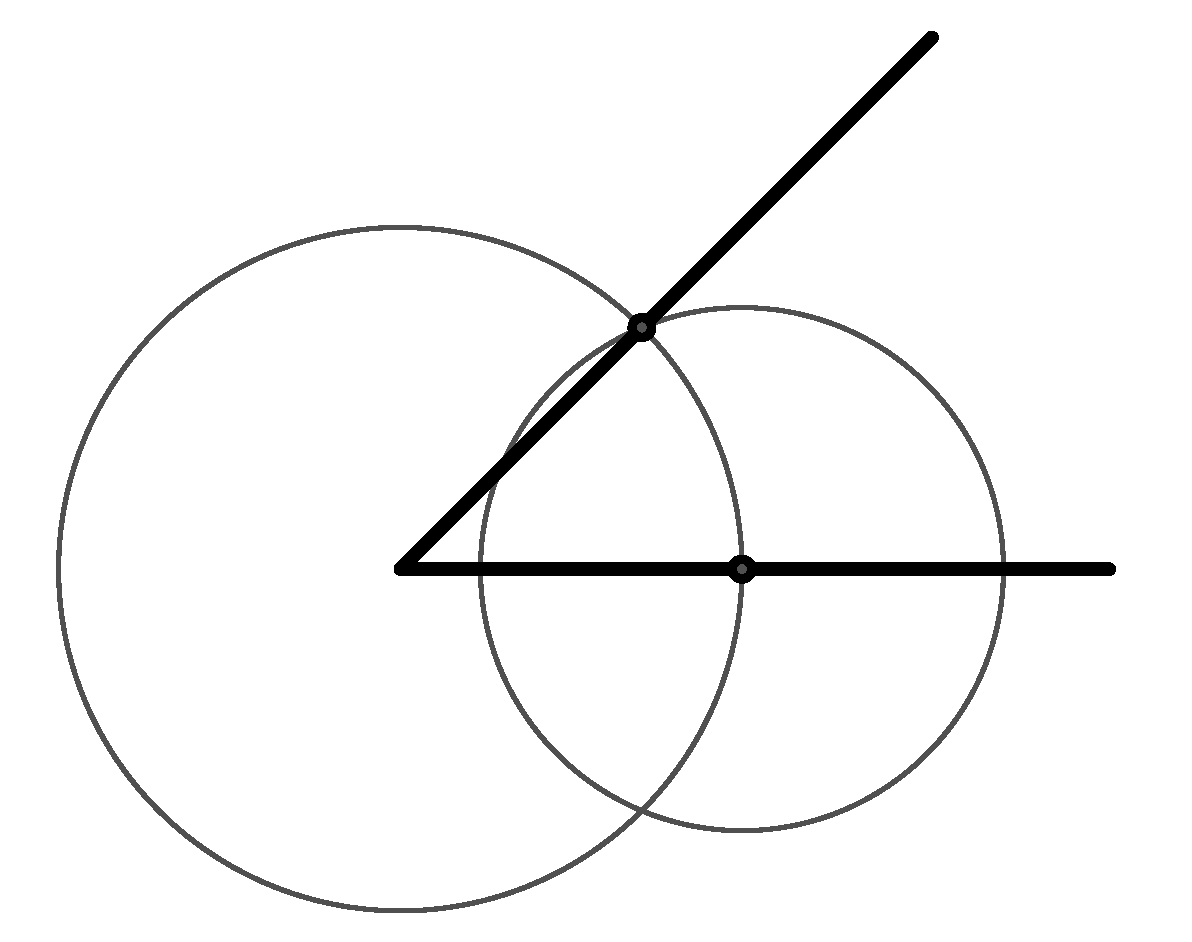
\includegraphics{copyangle.png}
%\end{image}
\end{hint}
\end{freeResponse}
\end{problem}


\begin{problem}
Construct a $30$-$60$-$90$ right triangle. Explain the steps in your
  construction and how you know it works.
\begin{freeResponse}
\begin{hint}
Construct an equilateral triangle and cut it in half.  
\end{hint}
\end{freeResponse}
\end{problem}

\begin{problem}
Construct an isosceles right triangle. Explain the steps in your
  construction and how you know it works.
\begin{freeResponse}
\begin{hint}
Construct a square and draw a diagonal.  
\end{hint}
\end{freeResponse}
\end{problem}



\end{document}
